\section{Problem 2}

In this problem we analyse the Vandermonde matrix and use various techniques to solve it. The way I formatted this is by first listing the whole code, and then per sub-question discussing the output of relevant part of the code. I did this because some of the code overlaps between sub-questions. Per sub-question, I indicate in the code the part relevant to it (e.g. \#2A). The code I have written is as follows: 

\lstinputlisting{NURhandin1_2.py}

\subsection{Problem 2a}

First we take a look at problem 2a. In this problem, the goal is to write a code that does an LU decomposition of the Vandermonde matrix and use the resulting LU matrix to obtain the solutions $c_i$ for data points $x_i$, where i = 0,1,...,19. First of all, we create the matrix V. We do this by taking every row to be (1, $x_i$, $x_{i}^2$, ...., $x_{i}^{19}$), again for our different 20 data values $x_i$, filling j = 1,2,...,19 rows in total. In order to first obtain the LU matrix, we apply the Improved Crout's algorithm from lecture 3 slide 15 as shown in the code. As can be seen in the code, we first take our LU matrix as the input matrix V (as instructed on slide 13), and gradually swap and overwrite different elements of the matrix. All used for loops can be translated to summing for different values i within the range of the loop. The if-statements determine the conditions for which we should apply operations. After we finish all loops, we return a matrix LU of equivalent shape to V that contains our $\alpha_{ij}$ and $\beta_{ij}$ values, which we will require to apply forward- and backward substitution.\\

Next, using the LU matrix and the given b=$y_i$ data values, we apply a forward subtitution algorithm inspired by slide 11 of lecture 3. The diving by $\alpha_{ii}$ factors are omitted because we have set these values to be equal to 1 implicitly. From this rather straightforward algorithm, we (confusingly) obtain the y values we require to apply backward subtitution. This algorithm is a bit more complicated. We go through this loop in reverse order, applying numerous operations to construct our solution vector x. These operations include dividing by $\beta_{ii}$ and multiplying by $\beta_{ij}$ and $y_i$ values respectively for j $>$ i, opposite from the conditions from the forward subtitution, j $<$ i. Finally, we combine these three seperate algorithms into a final function in which we can input the matrix we want to solve A and it's solution b. In our case, we will use V and y respectively for this. This function then returns a vector of x-values. These are the c-values we wished to obtain, given by:

\lstinputlisting{problem2a.txt}

The plots for this are:

\begin{figure}[h!]
  \centering
  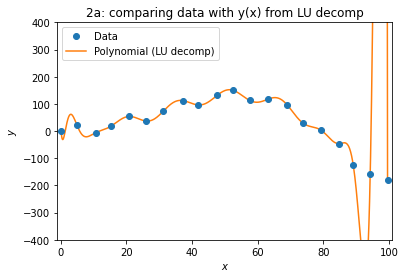
\includegraphics[width=0.6\linewidth]{problem2a1.png}
  \caption{The polynomial y(x) obtained with the LU decomposition method plotted together with the given data points to test whether it intersects them.}
  \label{fig:fig1}
\end{figure}

The other figure is: 

\begin{figure}[h!]
  \centering
  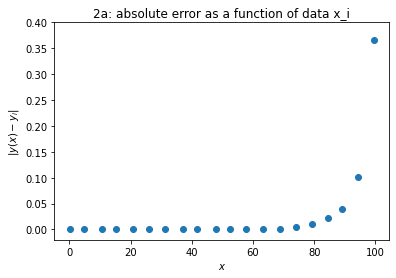
\includegraphics[width=0.6\linewidth]{problem2a2.png}
  \caption{The absolute difference between the polynomial y(x) and the data points $y_i$ to visualise how far off the polynomial is from the actual data. This y-scale seemed most appropiate as it still includes the point with the highest error value. Smaller y limit values barely show any error in the lower x values regardless.}
  \label{fig:fig2}
\end{figure}